\documentclass[14pt,compress]{beamer}
\usepackage[spanish]{babel}
\usepackage[utf8]{inputenc}
\usepackage{presento}
\usepackage{comment}

\makeatletter
\newcommand{\vast}{\bBigg@{4}}
\newcommand{\Vast}{\bBigg@{5}}
\makeatother

%configuration file
%\setbeamercolor{title}{fg=DarkRed}
%\setbeamercolor{frametitle}{fg=DarkRed}
\setbeamercolor{normal text}{fg=darkgray}
\usebeamercolor[fg]{normal text}
%\setbeamercolor{block title}{fg=black,bg=Fern!25!white}
%\setbeamercolor{block body}{fg=black,bg=Fern!25!white}
%\setbeamercolor{alerted text}{fg=AlertColor}
%\setbeamercolor{itemize item}{fg=Charcoal}

\usepackage[font={color=dimgray},figurename={ },labelfont={ }]{caption}

% personal data
\newcommand{\mycongress}{\setnote{\color{darkgray}\small
I Encuentro Nacional de Din\'amica Cu\'antica en la Materia}}
\newcommand{\myTitle}{\color{orange}{\fontsize{27}{29}\selectfont 
Implementación de Métodos de Aprendizaje Automatizado
en problemas colisionales}}
\newcommand{\myemail}{\setnote{\color{darkgray}\scriptsize 
alemendez@iafe.uba.ar}}
\newcommand{\myDetails}{\setnote{\color{darkgray}\small 
1 de Septiembre -- Buenos Aires}}

% colors: black, blue, brown, cyan, darkgray, gray, green, 
% lightgray, lime, magenta, olive, orange, pink, purple, red, teal, 
% violet, white, yellow.

\begin{document}
%%%%%%%%%%%%%%%%%%%%%%%%%%%%%%%%%%%%%%%%%%%%%%%%%%%%%%%%%%%%%%%%%
\begin{frame}[plain]
\vfill
\mycongress

\vspace{0.7cm}
\myTitle
% \hline

\noindent\makebox[\linewidth]{\rule{0.85\paperwidth}{0.7pt}}
\vfill

% \vspace{0.5cm}
\hspace{2.75cm}\text{\color{teal}{\normalsize Alejandra Mendez,}} \\
\hspace{2.75cm}\text{\color{teal}{\normalsize Juan Di Filippo,}} \\
\hspace{2.75cm}\text{\color{teal}{\normalsize Sebasti\'an L\'opez,}} \\
\hspace{2.75cm}\text{\color{teal}{\normalsize Dar\'io Mitnik,}} \\
\vfill
\vspace{-0.25cm}
\hspace{2.5cm}\myemail
\vfill
\begin{tikzpicture}[remember picture,overlay]
\node[xshift=-10.7cm,yshift=-6.45cm] at (current page.north east) 
{
\includegraphics[width=0.28\textwidth]{iafe.jpg}};
\end{tikzpicture}

\vspace{-0.5cm}
\centering
\myDetails 

\end{frame}
%%%%%%%%%%%%%%%%%%%%%%%%%%%%%%%%%%%%%%%%%%%%%%%%%%%%%%%%%%%%%%%%%%%%%%%%
\section{Machine Learning}
%%%%%%%%%%%%%%%%%%%%%%%%%%%%%%%%%%%%%%%%%%%%%%%%%%%%%%%%%%%%%%%%%%%%%%%%
\framepic[1.]{figures/mlcover_modif.png}{
 \begin{textblock}{8}(6.5,-2.2)
    {\color{orange0}
\text{\huge \bf Machine} \\
\vspace{2pt}
\text{\huge\bf Learning}}
 \end{textblock}}
%%%%%%%%%%%%%%%%%%%%%%%%%%%%%%%%%%%%%%%%%%%%%%%%%%%%%%%%%%%%%%%%%%%%%%%%
%%%%%%%%%%%%%%%%%%%%%%%%%%%%%%%%%%%%%%%%%%%%%%%%%%%%%%%%%%%%%%%%%%%%%%%%
\framepic[1.]{figures/ionization.png}{}
%%%%%%%%%%%%%%%%%%%%%%%%%%%%%%%%%%%%%%%%%%%%%%%%%%%%%%%%%%%%%%%%%%%%%%%%
\section{DIM}
%%%%%%%%%%%%%%%%%%%%%%%%%%%%%%%%%%%%%%%%%%%%%%%%%%%%%%%%%%%%%%%%%%%%%%%%
\begin{frame}
\frametitle{Método de Inversión Depurada (DIM)}

\vspace{-1.5cm}
\begin{equation*}
\tikzmarkin[draw=darkgray,fill=darkgray!10]{potencial}(0.2,-0.3)(-0.1,0.65)
T_{fi} = \big| \langle \psi_f |  V 
| \psi_i \rangle \big|^2 
\tikzmarkend{potencial}
\end{equation*}
\begin{tikzpicture}[remember picture, overlay,
  expl1/.style={draw=red,fill=orange!7,rounded corners,text width=3cm,
  minimum width=1.2cm, minimum height=0.7cm, text centered},
  arrow/.style={red,ultra thick,->,>=latex}
  ]
\node<2->[expl1] (potexp) at (9.5cm,2cm) {\color{orange-red}{¿Cómo obtener V?}};
\draw<2->[arrow, bend right=30, dashed] ([xshift=0cm,yshift=0cm]{potexp.west}) to
         ([xshift=2.5cm,yshift=-0.2cm]{potencial});  
\node<3> (schro) at (5cm,-1cm)
{$ \left[ -\frac{1}{2} \frac{d^2}{d r^2} + \frac{l(l+1)}{2 r^2} 
+ V_{nl}(r) \right] \, P_{nl}(r) = 
E_{nl} \, P_{nl}(r) $};
\node<4-> (schro) at (5cm,-1cm)
{$ \left[ -\frac{1}{2} \frac{d^2}{d r^2} + \frac{l(l+1)}{2 r^2} 
- \frac{Z_{nl}(r)}{r} \right] \, P_{nl}(r) = 
E_{nl} \, P_{nl}(r) $};
\node<5-> (znl) at (5cm,-2.5cm)
{$ Z_{nl}(r) = -\frac{1}{2} 
\frac{P_{nl}''(r)}{ P_{nl}(r)} \,r
+ \frac{l(l+1)}{2 r} - E_{nl} \,r $};
\end{tikzpicture}

\end{frame}
%%%%%%%%%%%%%%%%%%%%%%%%%%%%%%%%%%%%%%%%%%%%%%%%%%%%%%%%%%%%%%%%%%%%%%%%
\begin{frame}
\frametitle{Houston, we have a problem!}

\vspace{-0.25cm}
\begin{tikzpicture}
  \node (img1) 
  {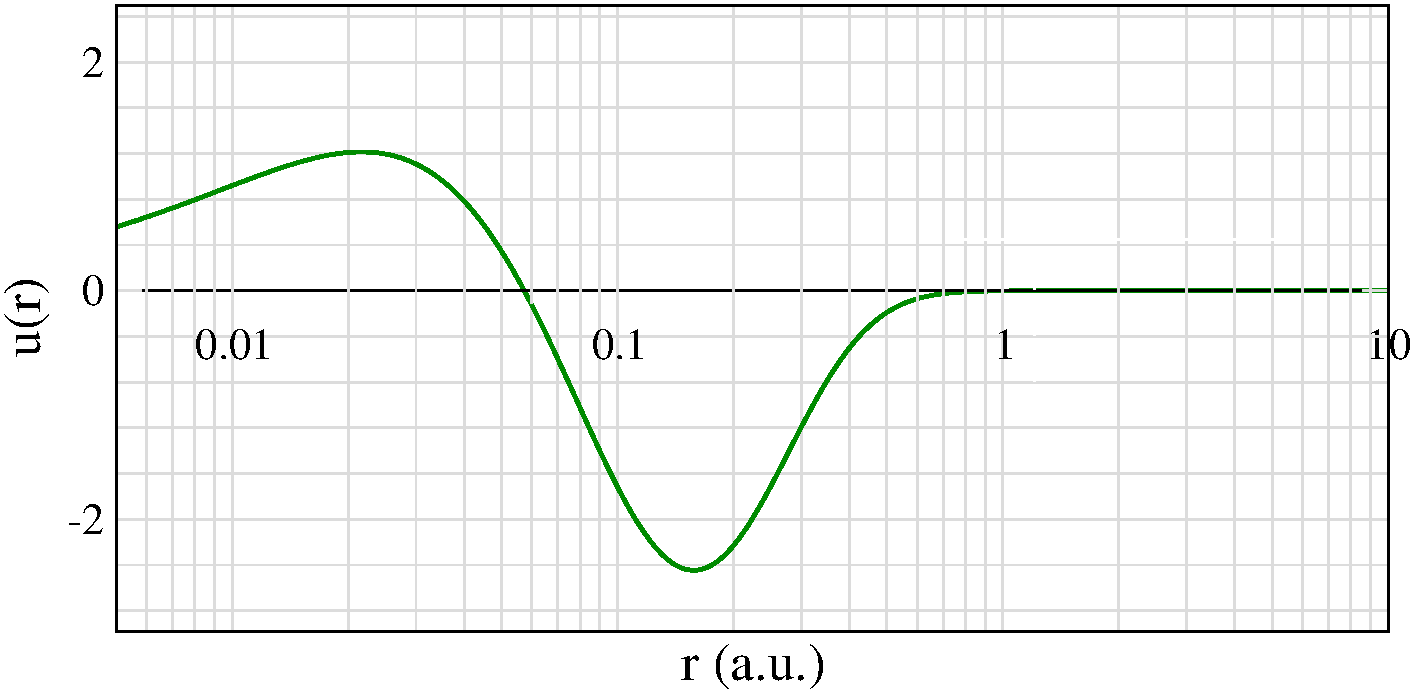
\includegraphics[width=0.95\textwidth]{figures/dim/wavefun2sKr.pdf}};
%  \node<1-> (eq1) at (img1) [yshift=1.4cm,xshift=1.5cm]
%  {$Z(r) = -\frac{1}{2} \frac{P''(r)}{P(r)} \,r  - E \, r$}; 
  \node (eq2) at (img1) [yshift=3cm,xshift=4cm] 
  {{\normalsize $2s$ Kr}}; 
  \node<2-> (img2) at (img1.west) [xshift=2cm,yshift=-2.25cm]
  {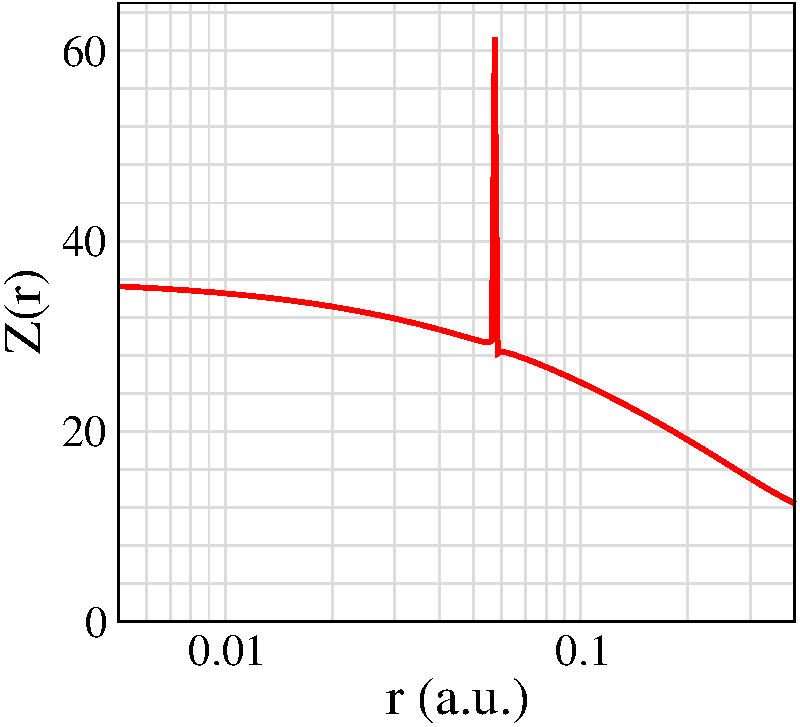
\includegraphics[width=0.4\textwidth]{figures/dim/problem1-2sKr.pdf}};
  \node<3-> (img3) at (img1.east) [xshift=-1.75cm,yshift=-2.25cm]
  {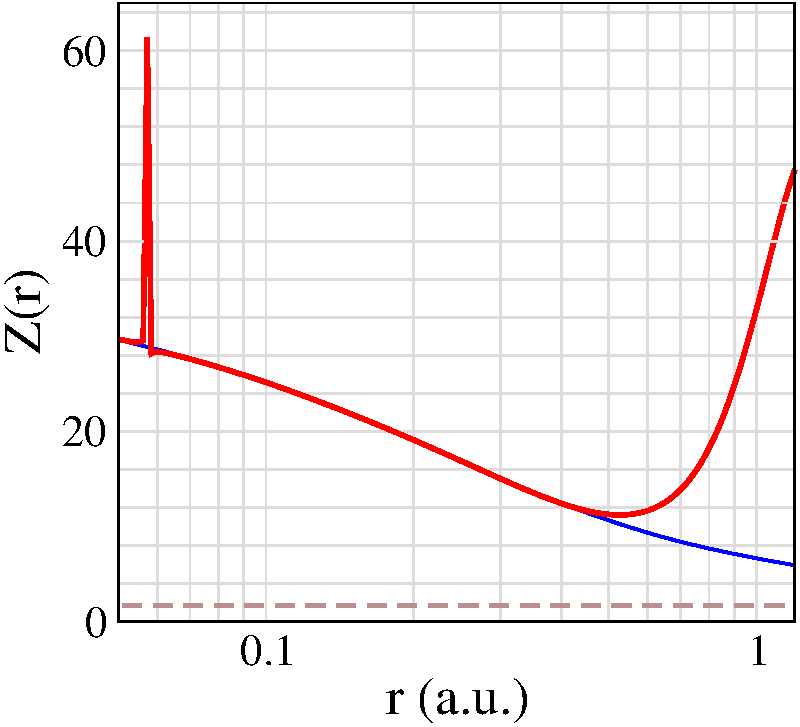
\includegraphics[width=0.4\textwidth]{figures/dim/problem2-2sKr.pdf}};
\end{tikzpicture}

\end{frame}
%%%%%%%%%%%%%%%%%%%%%%%%%%%%%%%%%%%%%%%%%%%%%%%%%%%%%%%%%%%%%%%%%%%%%%%%
\begin{frame}
\frametitle{Depuraci\'on}

\begin{tikzpicture}[remember picture,overlay]
  \tikzset{shift={(current page.center)}}%xshift=-1.5cm,yshift=0cm}
  \node (img1) 
  {\includegraphics[width=0.7\textwidth]{figures/dim/depuration2sN-a.eps}};
  \node (name) at (img1) [yshift=2.9cm,xshift=2.8cm] 
  {$2s$ N};
  \node<3-> (eq1) at (img1) [yshift=-3.5cm,xshift=0cm]
  {$\tikzmarkin[draw=orange,fill=orange!10]{depuration}(0.2,-0.5)(-0.1,0.65)
   Z(r) = 1+\sum_{j} \alpha_j e^{-\beta_j r} 
   \tikzmarkend{depuration}$};
  \node<3-> (img2) 
  {\includegraphics[width=0.7\textwidth]{figures/dim/depuration2sN-b.eps}};
  \node<2-> (asym) at (img1) [yshift=0cm,xshift=-1.1cm]
  { {\small $\Bigg\{ \!\! \begin{array}{c}
  \!\!\!\!Z_N :\, r=0 \\ 
  \,1 \,\,\,:\, r\rightarrow \infty\\ \end{array} $ } };
  \node<4-> (eq1) at (img1) [yshift=-3.5cm,xshift=0cm]
  {$\tikzmarkin[draw=orange,fill=orange!10]{depuration}(0.21,-0.5)(-0.1,0.65)
   Z(r) = 1+\sum_{j} {\color{orange}{\mathbf{\boldsymbol\alpha_j}}} 
          e^{-{\color{orange}{\mathbf{\boldsymbol\beta_j}}} r} 
   \tikzmarkend{depuration}$};
\end{tikzpicture}

\end{frame}
%%%%%%%%%%%%%%%%%%%%%%%%%%%%%%%%%%%%%%%%%%%%%%%%%%%%%%%%%%%%%%%%%%%%%%%%
\begin{frame}
\frametitle{Procedimiento}

\begin{tikzpicture}[remember picture, overlay,
  expl1/.style={draw=red,fill=orange!7,rounded corners,text width=3cm,
  minimum width=0.5cm, minimum height=0.7cm, text centered},
  arrow/.style={red,ultra thick,->,>=latex}]
  \tikzset{shift={(current page.center)},xshift=0cm,yshift=2.5cm}
  \node[expl1,text width=2cm] (inv) {Inversión};
  \node[expl1,text width=5.4cm] (rem) at (inv) [xshift=0cm,yshift=-1.4cm]
  {Remoción de divergencias};
  \node[expl1,text width=2.75cm] (var) at (rem) [xshift=0cm,yshift=-1.8cm]
  {Variación de parámetros};
  \node[expl1,text width=3.1cm] (diag) at (var) [xshift=2.5cm,yshift=-2cm]
  {Diagonalización};
  \node[expl1,text width=3.3cm] (err) at (var) [xshift=-2.5cm,yshift=-2cm]
  {Calculo de error};
  \draw [arrow, bend right=0] 
  ([xshift=0cm,yshift=0cm]{inv}) to ([xshift=0cm,yshift=0cm]{rem.north});
  \draw [arrow, bend right=0] 
  ([xshift=0cm,yshift=0cm]{rem}) to ([xshift=0cm,yshift=0cm]{var.north});
  \draw [arrow, bend right=-30] 
  ([xshift=0cm,yshift=0cm]{var.east}) to ([xshift=0cm,yshift=0cm]{diag.north});
  \draw [arrow, bend right=-40] 
  ([xshift=0cm,yshift=0cm]{diag}) to ([xshift=0cm,yshift=0cm]{err.south});
  \draw [arrow, bend right=-30] 
  ([xshift=0cm,yshift=0cm]{err}) to ([xshift=0cm,yshift=0cm]{var.west});
  \draw [arrow, bend right=-30,dashed] 
  ([xshift=-0.75cm,yshift=0cm]{err.north}) to ([xshift=0cm,yshift=-0.25cm]{rem.west});
\end{tikzpicture}

\end{frame}
%%%%%%%%%%%%%%%%%%%%%%%%%%%%%%%%%%%%%%%%%%%%%%%%%%%%%%%%%%%%%%%%%%%%%%%%
\section{R--Matrix}
%%%%%%%%%%%%%%%%%%%%%%%%%%%%%%%%%%%%%%%%%%%%%%%%%%%%%%%%%%%%%%%%%%%%%%%%
\begin{frame}
\frametitle{R--Matrix}

\begin{columns}
\begin{column}{0.55\textwidth}
\begin{center}
\begin{figure}
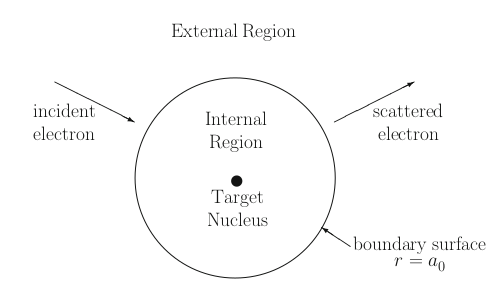
\includegraphics[width=\textwidth]{figures/theoryRM/regions.png}
\end{figure}
\end{center}
\end{column}
\begin{column}{0.45\textwidth}  %%<--- here
\begin{tikzpicture}[remember picture,overlay,
  arrow/.style={red,ultra thick,->,>=latex}]
  \tikzset{shift={(current page.center)},xshift=2.9cm,yshift=2.25cm}
  \node (target) {Estructura del blanco};
  \node (auto) at (target) [xshift=0cm,yshift=-0.65cm] {\fbox{\sc \small autostructure}};
%
  \node (inner) at (target) [xshift=0cm,yshift=-2.25cm] {Región interna};
  \node (rmatrxi) at (inner) [xshift=0cm,yshift=-0.65cm] {\fbox{\sc \small rmatrxi}};
%
  \node (outer) at (inner) [xshift=0cm,yshift=-2.25cm] {Región externa};
  \node (stgf) at (outer) [xshift=0cm,yshift=-0.65cm] {\fbox{\sc \small stgf}};
%
  \draw [arrow, bend right=0] (auto) to ([xshift=0cm,yshift=0cm]{inner.north});
  \draw [arrow, bend right=0] (rmatrxi) to ([xshift=0cm,yshift=0cm]{outer.north});
\end{tikzpicture}

\end{column}
\end{columns}


\end{frame}
%%%%%%%%%%%%%%%%%%%%%%%%%%%%%%%%%%%%%%%%%%%%%%%%%%%%%%%%%%%%%%%%%%%%%%%%
\begin{frame}
\frametitle{Descripción del blanco}

\begin{tikzpicture}[remember picture,overlay]
  \tikzset{shift={(current page.center)},xshift=0cm,yshift=1.5cm}
  \node (eqCI) 
  {$\tikzmarkin[draw=orange,fill=orange!10]{ci}(0.1,-0.4)(-0.1,0.65)
    \Phi_i(\mathbf{r}) = \sum_j c_{ji} \phi_j(\mathbf{r})
    \tikzmarkend{ci}$};
  \node (name) at (eqCI) [xshift=4.cm,yshift=0cm]
  {$\begin{array}{c}
     \mbox{\small Configuration} \\
     \mbox{\small interaction}
   \end{array}$};
  \node (pnl) at (eqCI) [xshift=0cm,yshift=-1.75cm]
   {$\left[ \frac{1}{2} \frac{d^2}{dr^2} - \frac{l(l+1)}{2r^2} 
     + V_{nl}^{\mbox{\scriptsize eff}}(\lambda_{nl},r) + E_{nl} \right] 
     P_{nl}(r)=0$};
  \node (pot) at (pnl) [xshift=-2cm,yshift=-2cm]
  {{\begin{varwidth}{\linewidth}
     \begin{itemize}
        \item Thomas–Fermi–Dirac–Amaldi 
        \item Slater-Type-Orbital de Burgess  
     \end{itemize}
    \end{varwidth}}}; 
\end{tikzpicture}

\end{frame}
%%%%%%%%%%%%%%%%%%%%%%%%%%%%%%%%%%%%%%%%%%%%%%%%%%%%%%%%%%%%%%%%%%%%%%%%
\begin{frame}
\frametitle{Ejemplo: Berilio}
\begin{tikzpicture}[remember picture,overlay]
  \tikzset{shift={(current page.center)},xshift=0.5cm,yshift=0cm}
  \node<-1> (be_config) 
  {\includegraphics[width=0.7\textwidth]{figures/theoryRM/example_conf.eps}};
  \node<-1> (be_ecfgs) at (be_config) [xshift=-5.25cm,yshift=1.5cm]
  {\small$ 
    \begin{array}{l}
      1s^2 2s^2 \\
      1s^2 2snl \\
      1s^2 2p^2 \\
      1s^2 2pnl \\
    \end{array}\!\vast\} $};
  \node<2> (be_levels) at (be_config) [xshift=-0.5cm,yshift=0cm]
  {\includegraphics[width=0.8\textwidth]{figures/theoryRM/Be_levels.eps}};
  \node<3-> (be_var) at (be_config) [xshift=-0.5cm,yshift=0cm]
  {\includegraphics[width=0.7\textwidth]{figures/theoryRM/example_var.eps}};
\end{tikzpicture}

\end{frame}
%%%%%%%%%%%%%%%%%%%%%%%%%%%%%%%%%%%%%%%%%%%%%%%%%%%%%%%%%%%%%%%%%%%%%%%%
\begin{frame}
\frametitle{Procedimiento}

\begin{tikzpicture}[remember picture, overlay,
  expl1/.style={draw=red,fill=orange!7,rounded corners,text width=3cm,
  minimum width=0.5cm, minimum height=0.7cm, text centered},
  arrow/.style={red,ultra thick,->,>=latex}]
  \tikzset{shift={(current page.center)},xshift=0cm,yshift=1.75cm}
  \node[expl1,text width=5.3cm] (defcfg) 
  {$\begin{array}{c}
   \mbox{Definición de} \\
   \mbox{configuración electrónica} \\
    \end{array}$};
  \node[expl1,text width=2.75cm] (var) at (rem) [xshift=0cm,yshift=-1.8cm]
  {Variación de parámetros};
  \node[expl1,text width=3.1cm] (diag) at (var) [xshift=2.5cm,yshift=-2cm]
  {Diagonalización};
  \node[expl1,text width=3.3cm] (err) at (var) [xshift=-2.5cm,yshift=-2cm]
  {Calculo de error};
  \draw [arrow, bend right=0] 
  ([xshift=0cm,yshift=0cm]{defcfg}) to ([xshift=0cm,yshift=0cm]{var.north});
  \draw [arrow, bend right=-30] 
  ([xshift=0cm,yshift=0cm]{var.east}) to ([xshift=0cm,yshift=0cm]{diag.north});
  \draw [arrow, bend right=-40] 
  ([xshift=0cm,yshift=0cm]{diag}) to ([xshift=0cm,yshift=0cm]{err.south});
  \draw [arrow, bend right=-30] 
  ([xshift=0cm,yshift=0cm]{err}) to ([xshift=0cm,yshift=0cm]{var.west});
  \draw [arrow, bend right=-30,dashed] 
  ([xshift=-0.75cm,yshift=0cm]{err.north}) to ([xshift=0cm,yshift=-0.25cm]{defcfg.west});
\end{tikzpicture}

\end{frame}
%%%%%%%%%%%%%%%%%%%%%%%%%%%%%%%%%%%%%%%%%%%%%%%%%%%%%%%%%%%%%%%%%%%%%%%%
\begin{frame}
\frametitle{Síntesis del problema}

\begin{equation*}
 J = \sum_j \left|\frac{E_j^{\mbox{\small calc}}(\boldsymbol{\xi}) 
- E_j^{\mbox{\small teo}}}{E_j^{\mbox{\small teo}}} \right|
\end{equation*}

\bigskip
\begin{itemize}
\item DIM: $\boldsymbol{\xi}=\{\boldsymbol{\alpha},\boldsymbol{\beta} \}$
\item R--Matrix: $\boldsymbol{\xi}=\{ Configuraciones,\boldsymbol{\lambda} \}$
\end{itemize}

\end{frame}
%%%%%%%%%%%%%%%%%%%%%%%%%%%%%%%%%%%%%%%%%%%%%%%%%%%%%%%%%%%%%%%%%%%%%%%%
\section{Procesos Gaussianos}
%%%%%%%%%%%%%%%%%%%%%%%%%%%%%%%%%%%%%%%%%%%%%%%%%%%%%%%%%%%%%%%%%%%%%%%%
\begin{frame}
\frametitle{Procesos Gaussianos}

\begin{tikzpicture}[remember picture, overlay]
  \tikzset{shift={(current page.center)},xshift=0cm,yshift=-0.5cm}
  \node<1> (func) {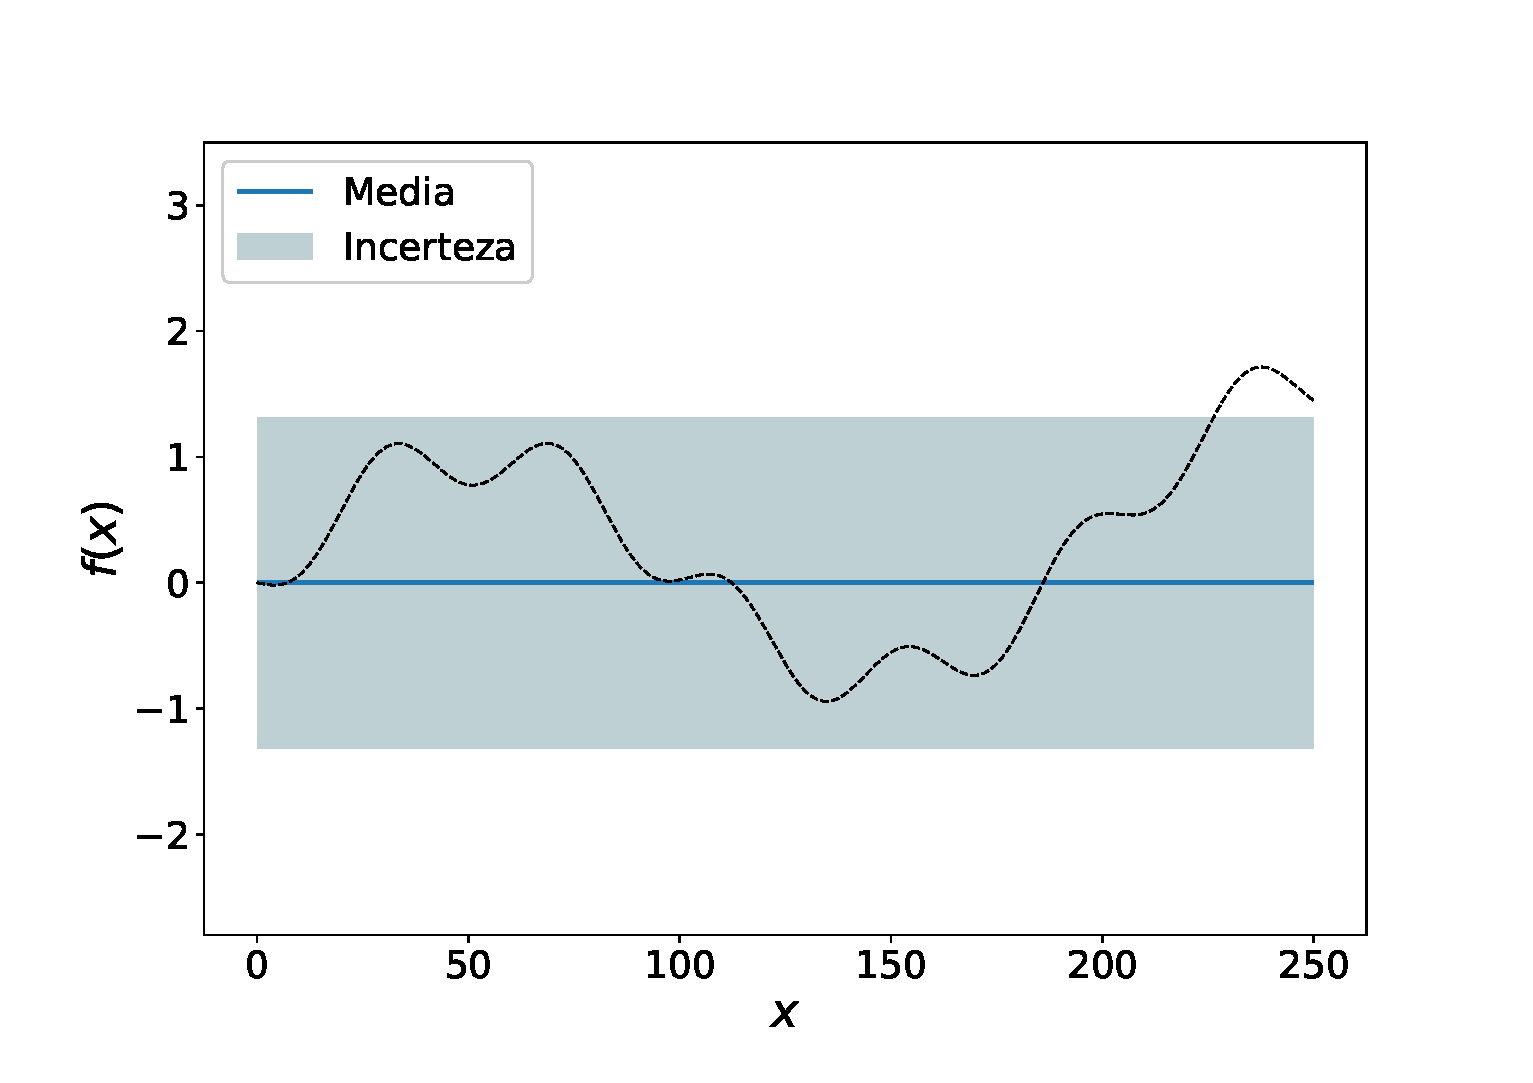
\includegraphics[width=\textwidth]{figures/gp/funcion.eps}};
  \node<2> (func) {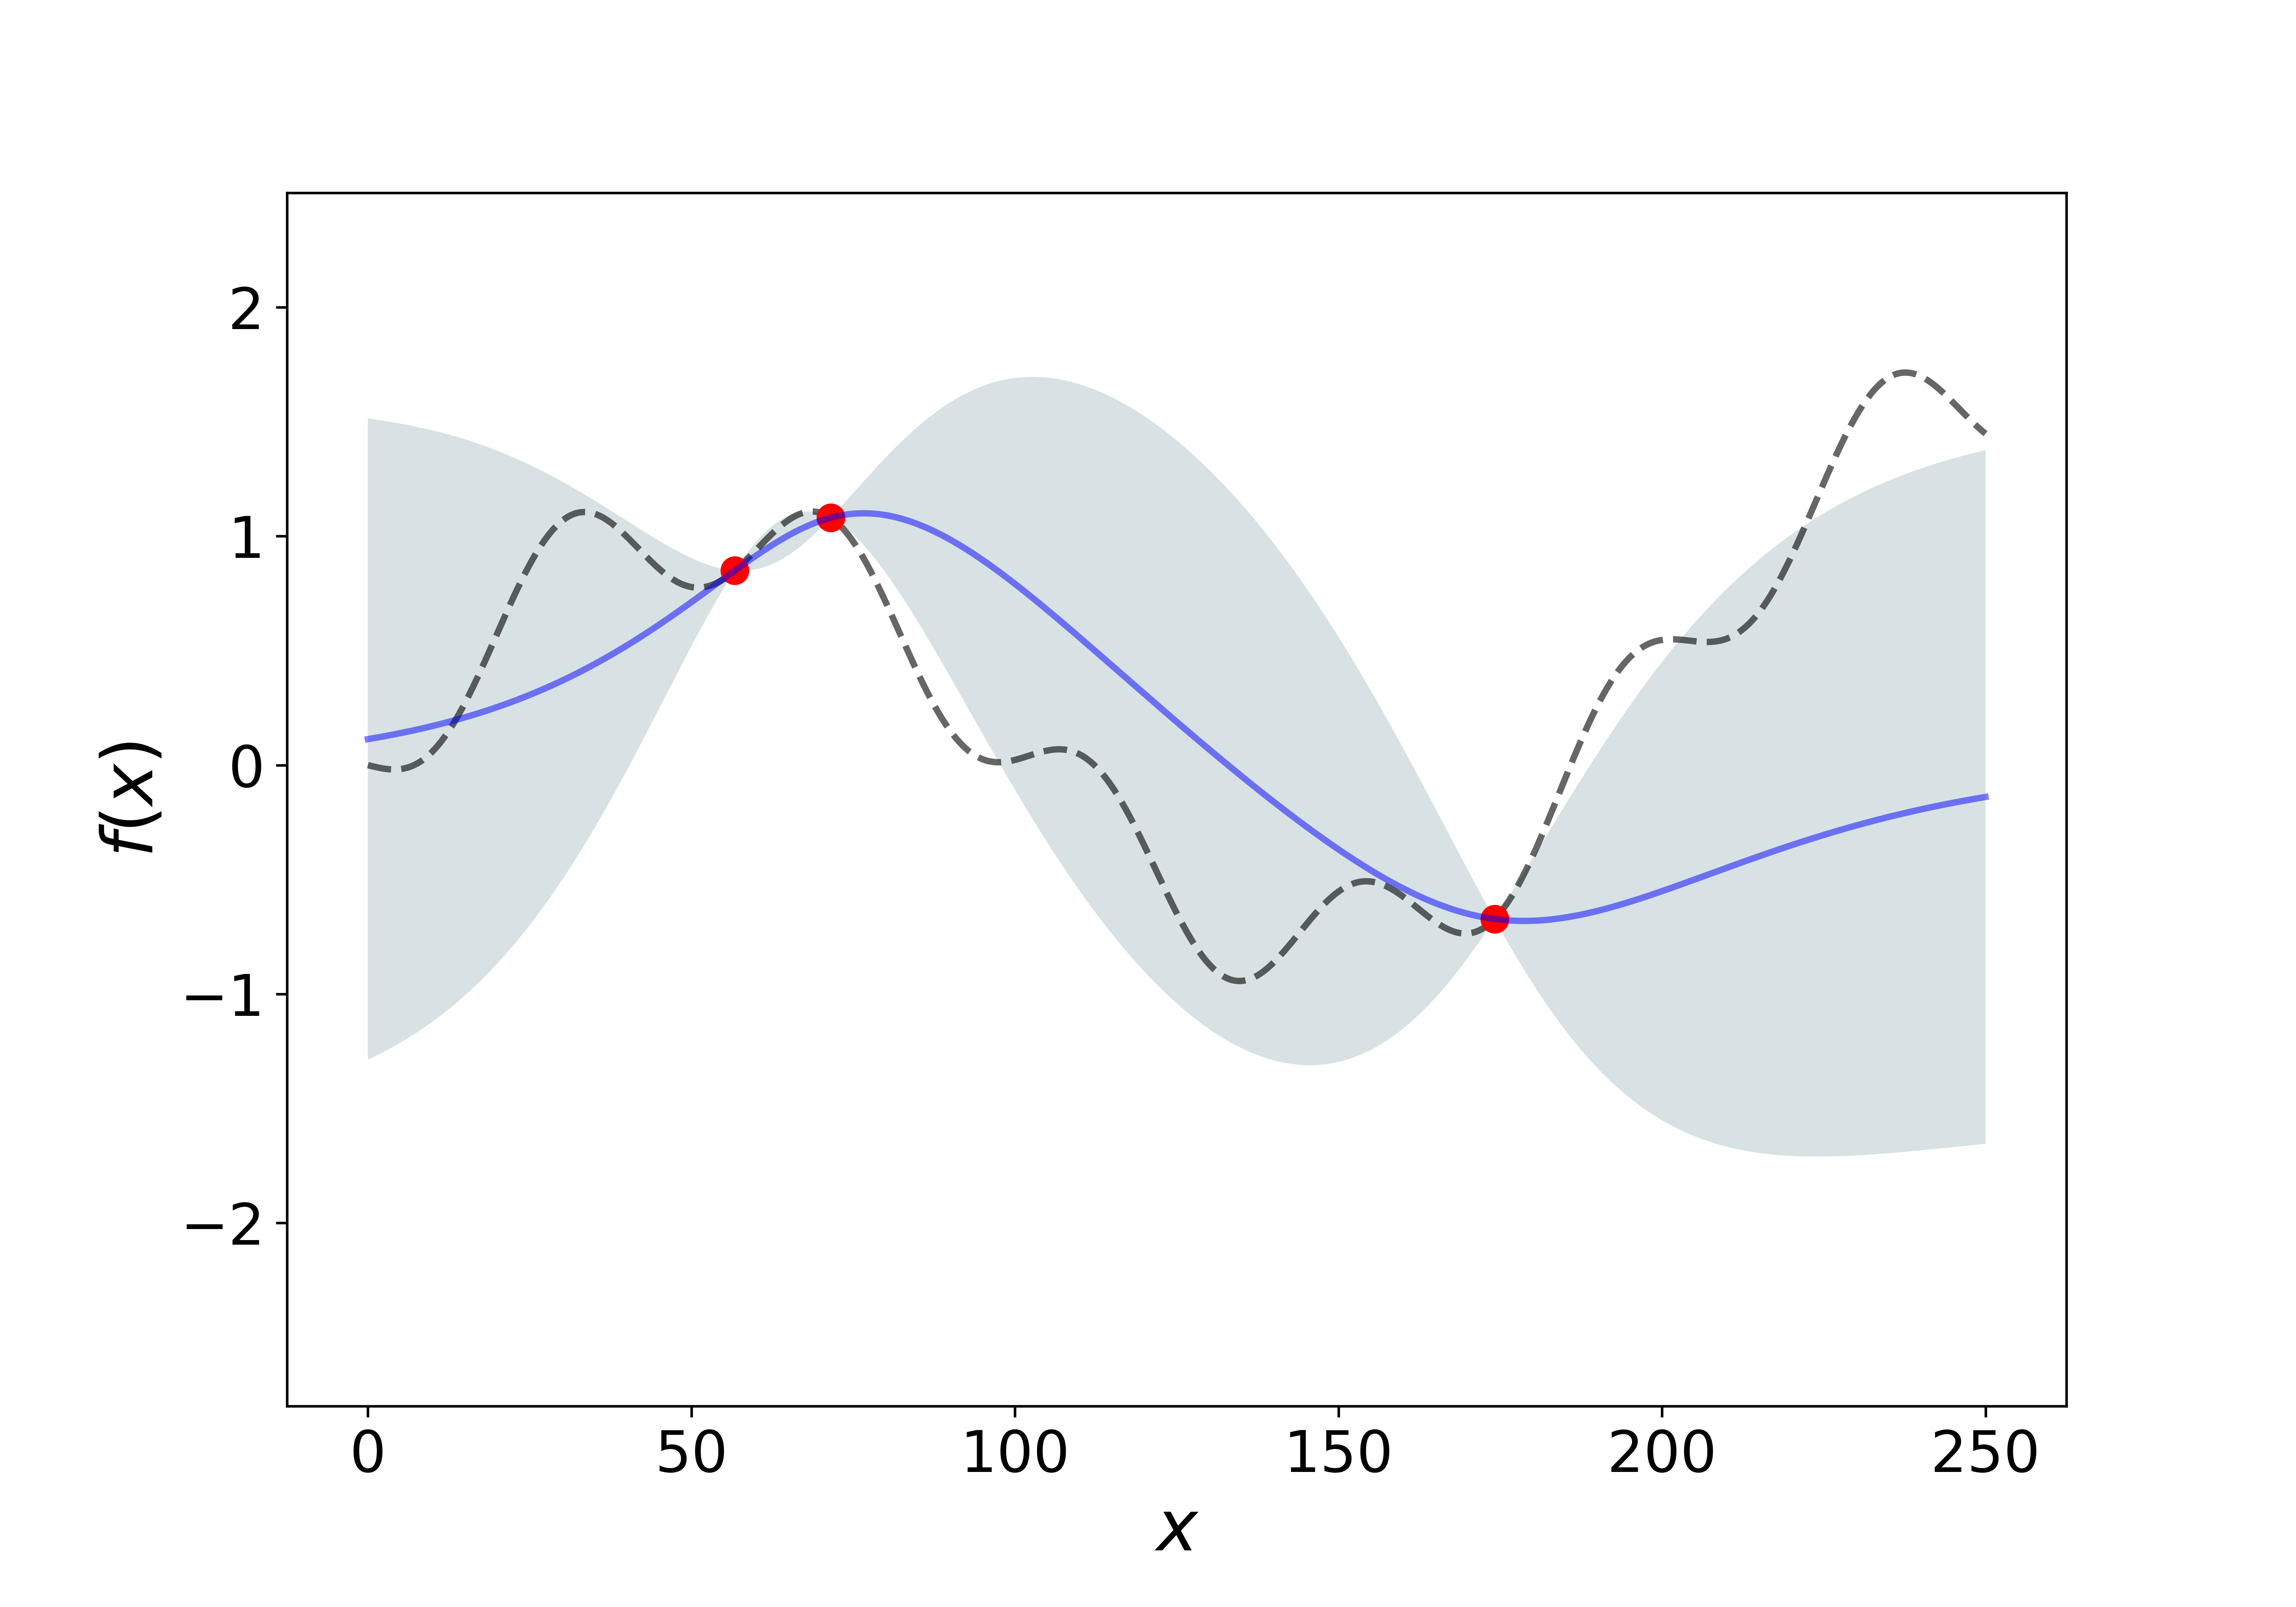
\includegraphics[width=\textwidth]{figures/gp/func_mean.eps}};
  \node<3> (func) {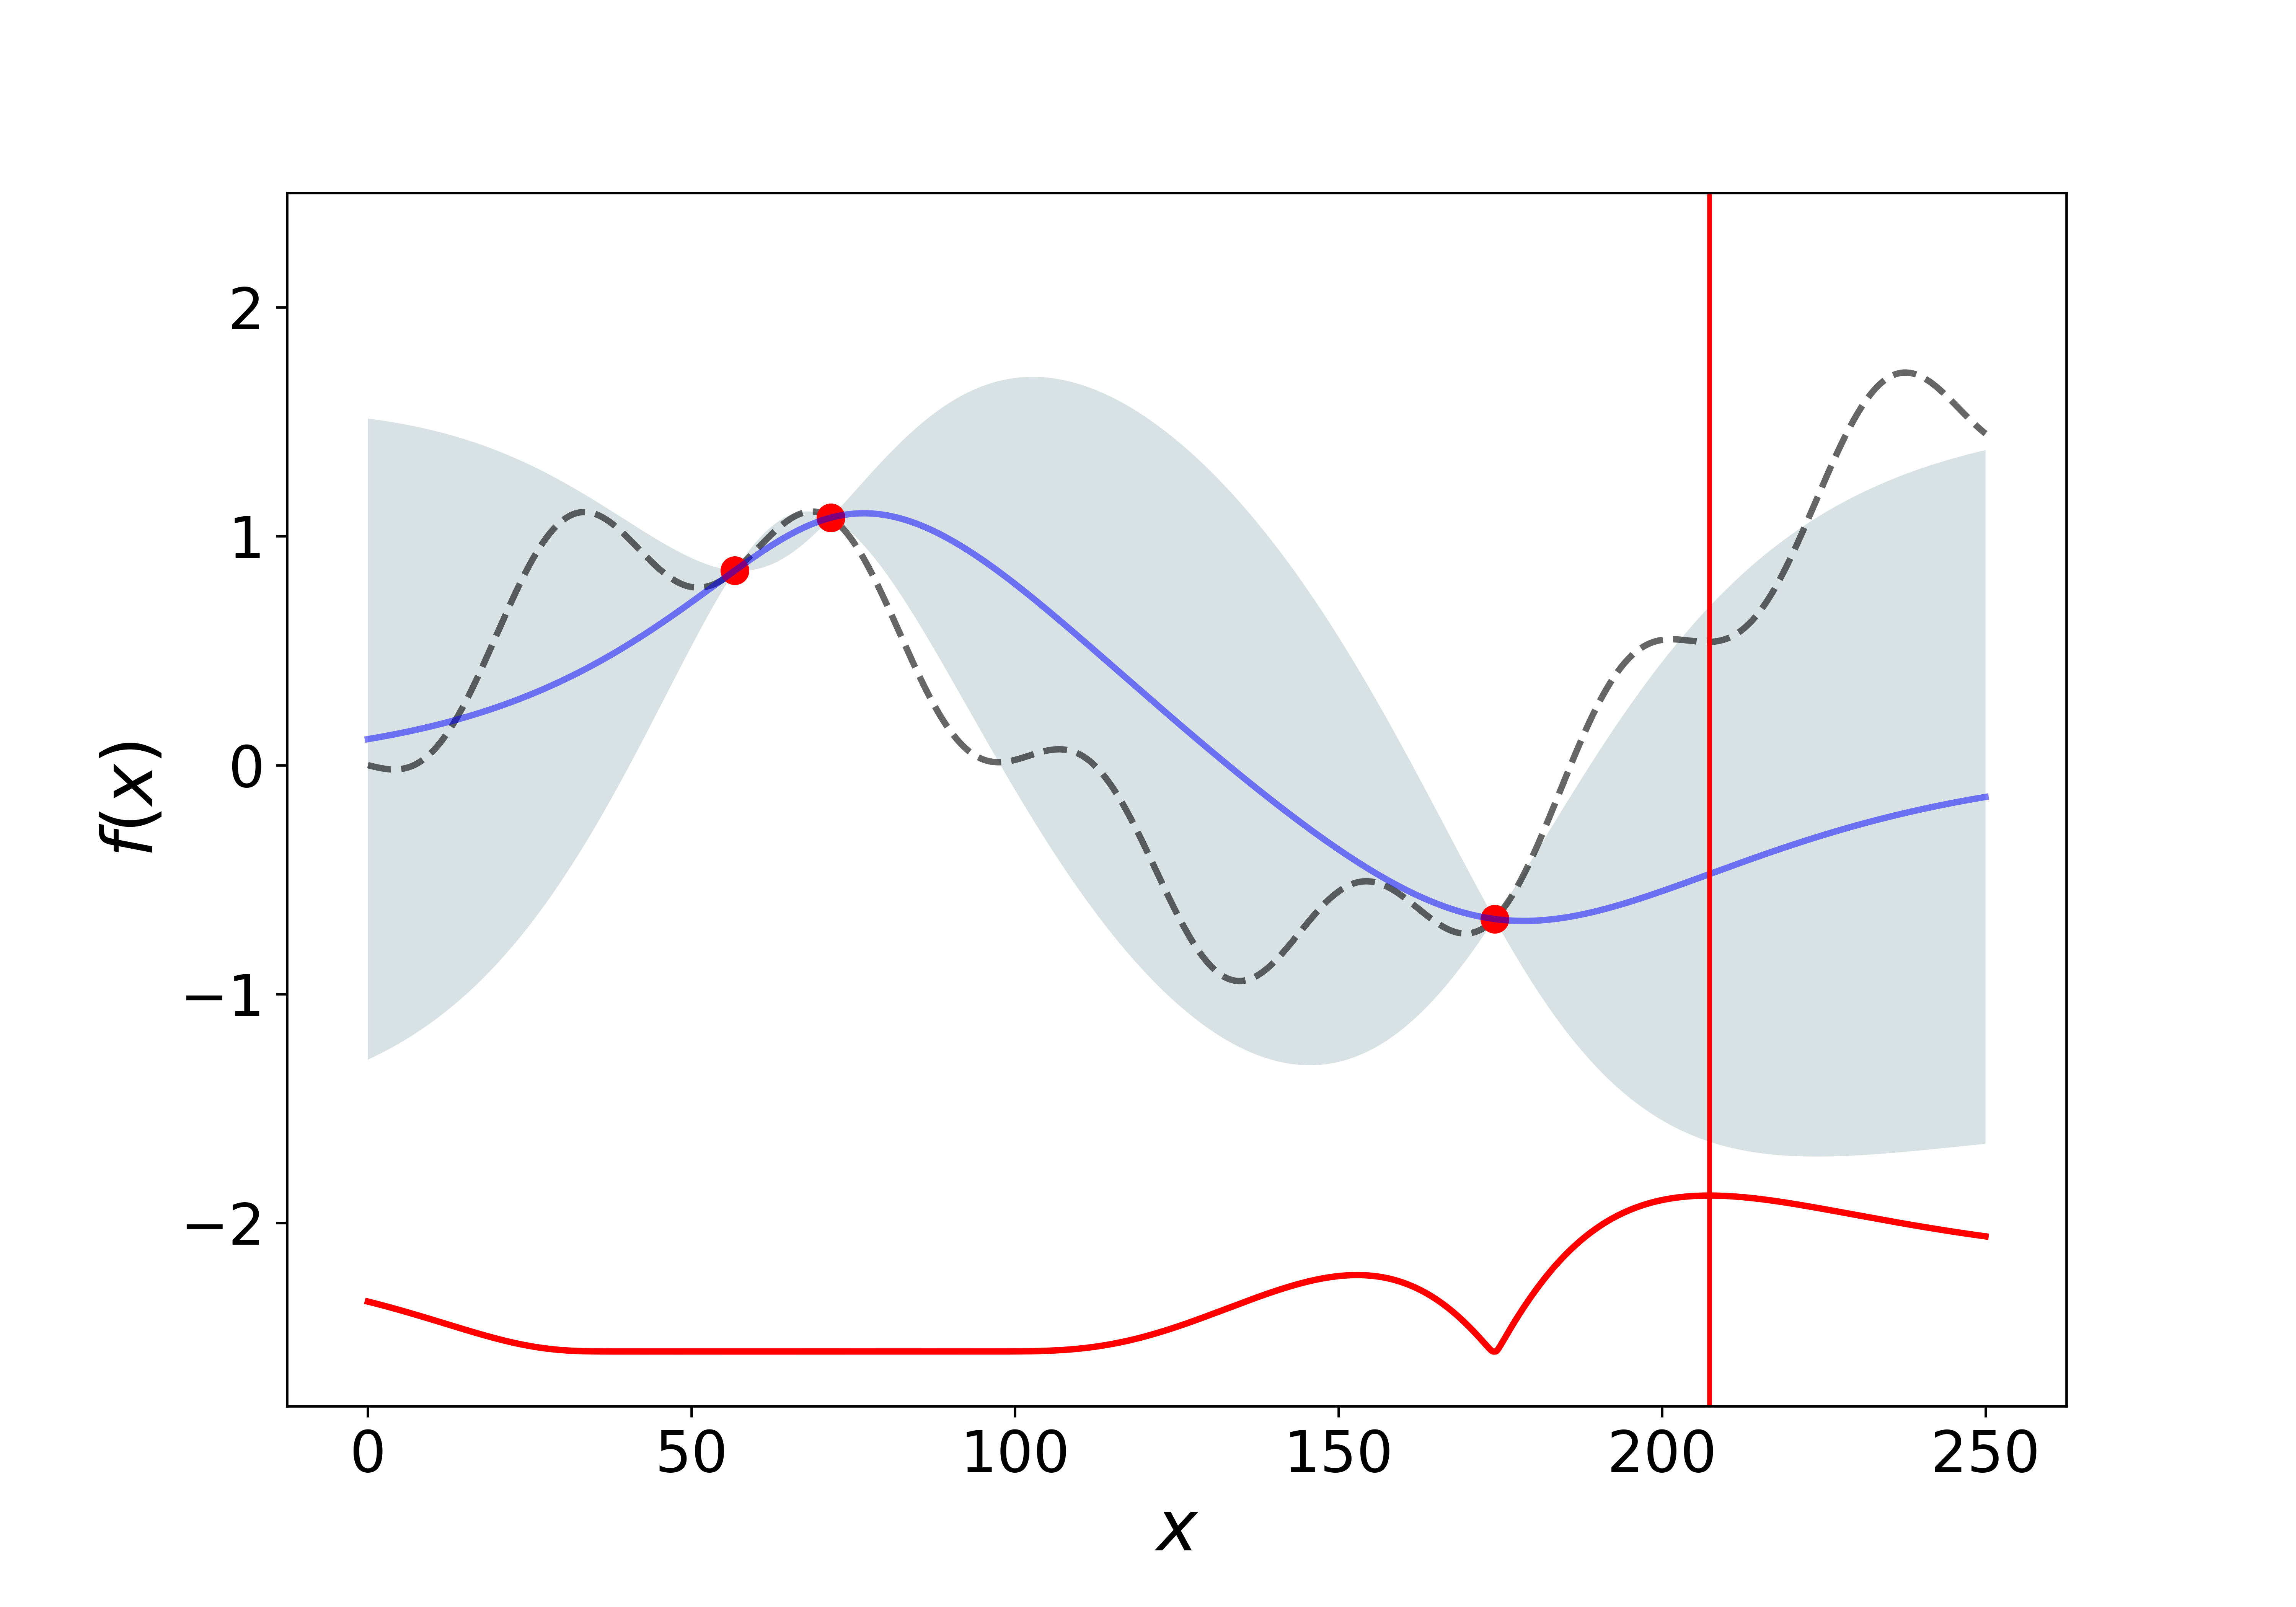
\includegraphics[width=\textwidth]{figures/gp/func_acq.eps}};
  \node<4> (max1) {\includegraphics[width=\textwidth]{figures/gp/eval1/example.eps}};
  \node<5> (max2) {\includegraphics[width=\textwidth]{figures/gp/eval2/example.eps}};
  \node<6> (max3) {\includegraphics[width=\textwidth]{figures/gp/eval3/example.eps}};
  \node<7> (max4) {\includegraphics[width=\textwidth]{figures/gp/eval4/example.eps}};
  \node<8> (max5) {\includegraphics[width=\textwidth]{figures/gp/eval5/example.eps}};
  \node<9> (max6) {\includegraphics[width=\textwidth]{figures/gp/eval6/example.eps}};
  \node<10> (max7) {\includegraphics[width=\textwidth]{figures/gp/eval7/example.eps}};
  \node<11> (max9) {\includegraphics[width=\textwidth]{figures/gp/eval8/example.eps}};
  \node<12> (max10) {\includegraphics[width=\textwidth]{figures/gp/eval9/example.eps}};
\end{tikzpicture}

\end{frame}
%%%%%%%%%%%%%%%%%%%%%%%%%%%%%%%%%%%%%%%%%%%%%%%%%%%%%%%%%%%%%%%%%%%%%%%%
\section{Resultados}
%%%%%%%%%%%%%%%%%%%%%%%%%%%%%%%%%%%%%%%%%%%%%%%%%%%%%%%%%%%%%%%%%%%%%%%%
\begin{frame}
\frametitle{DIM: Mg}

\begin{tikzpicture}[remember picture, overlay]
  \tikzset{shift={(current page.center)},xshift=-2.9cm,yshift=0.65cm}
  \node (1spot) 
  {\includegraphics[width=0.5\textwidth]{figures/dim/1s_pot.eps}};
  \node (tag) at (1spot) [xshift=7.25cm,yshift=2.75cm]
  {$1s$};
  \node (1swfn) at (1spot) [xshift=5.6cm,yshift=0cm]
  {\includegraphics[width=0.5\textwidth]{figures/dim/1s_wfn.eps}};
  \node (1serr) at (1spot) [xshift=5.6cm,yshift=-3.18cm]
  {\includegraphics[width=0.5\textwidth]{figures/dim/error_1s.eps}};
  \node (error) at (1spot) [xshift=0cm,yshift=-2.7cm]
  {$E \sim 10^{-6} $};
  \node (error) at (1spot) [xshift=0cm,yshift=-3.5cm]
  {$\langle r\rangle, \langle 1/r \rangle \sim 10^{-2} $};
\end{tikzpicture}

\end{frame}
%%%%%%%%%%%%%%%%%%%%%%%%%%%%%%%%%%%%%%%%%%%%%%%%%%%%%%%%%%%%%%%%%%%%%%%%
\begin{frame}
\frametitle{DIM: Mg}

\begin{tikzpicture}[remember picture, overlay]
  \tikzset{shift={(current page.center)},xshift=-2.9cm,yshift=0.65cm}
  \node (1spot) 
  {\includegraphics[width=0.5\textwidth]{figures/dim/2s_pot.eps}};
  \node (tag) at (1spot) [xshift=7.25cm,yshift=2.75cm]
  {$2s$};
  \node (1swfn) at (1spot) [xshift=5.58cm,yshift=0cm]
  {\includegraphics[width=0.505\textwidth]{figures/dim/2s_wfn.eps}};
  \node (1serr) at (1spot) [xshift=5.6cm,yshift=-3.11cm]
  {\includegraphics[width=0.5\textwidth]{figures/dim/error_2s.eps}};
  \node (error) at (1spot) [xshift=0cm,yshift=-2.7cm]
  {$E \sim 10^{-7} $};
  \node (error) at (1spot) [xshift=0cm,yshift=-3.5cm]
  {$\langle r\rangle, \langle 1/r \rangle \sim 10^{-2} $};
\end{tikzpicture}


\end{frame}
%%%%%%%%%%%%%%%%%%%%%%%%%%%%%%%%%%%%%%%%%%%%%%%%%%%%%%%%%%%%%%%%%%%%%%%%
\begin{frame}
\frametitle{DIM: Mg}

\begin{tikzpicture}[remember picture, overlay]
  \tikzset{shift={(current page.center)},xshift=-2.9cm,yshift=0.65cm}
  \node (1spot) 
  {\includegraphics[width=0.5\textwidth]{figures/dim/3s_pot.eps}};
  \node (tag) at (1spot) [xshift=7.25cm,yshift=2.75cm]
  {$3s$};
  \node (1swfn) at (1spot) [xshift=5.58cm,yshift=0cm]
  {\includegraphics[width=0.505\textwidth]{figures/dim/3s_wfn.eps}};
  \node (1serr) at (1spot) [xshift=5.6cm,yshift=-3.11cm]
  {\includegraphics[width=0.5\textwidth]{figures/dim/error_3s.eps}};
  \node (error) at (1spot) [xshift=0cm,yshift=-2.7cm]
  {$E \sim 10^{-5} $};
  \node (error) at (1spot) [xshift=0cm,yshift=-3.5cm]
  {$\langle r\rangle, \langle 1/r \rangle \sim 10^{-1} $};
\end{tikzpicture}


\end{frame}
%%%%%%%%%%%%%%%%%%%%%%%%%%%%%%%%%%%%%%%%%%%%%%%%%%%%%%%%%%%%%%%%%%%%%%%%
\begin{frame}
\frametitle{R--Matrix: Berilio}

\vspace{-0.2cm}
\begin{figure}
\includegraphics[width=0.4\textwidth]{figures/rmatrix/sig001-002.eps} 
\hspace{0.3cm}
\includegraphics[width=0.4\textwidth]{figures/rmatrix/sig001-003.eps} \\
\vspace{0.2cm}
\includegraphics[width=0.4\textwidth]{figures/rmatrix/sig001-006.eps} 
\hspace{0.3cm}
\includegraphics[width=0.4\textwidth]{figures/rmatrix/sig001-007.eps}
\end{figure}

\end{frame}
%%%%%%%%%%%%%%%%%%%%%%%%%%%%%%%%%%%%%%%%%%%%%%%%%%%%%%%%%%%%%%%%%%%%%%%%
\begin{frame}
\frametitle{Conclusiones}


\end{frame}
%%%%%%%%%%%%%%%%%%%%%%%%%%%%%%%%%%%%%%%%%%%%%%%%%%%%%%%%%%%%%%%%%%%%%%%%
\end{document}
